\section{Silniki 3D}
Mnogość źródeł jednoznacznie wskazuje, że gałąź jest dojrzała i oczekiwać można równie obfitej puli dostępnych rozwiązań.
Jest to w pełni prawidłowe założenie.
Rynek jest na tyle obszerny, że początkowo trudno zorientować się kto stanowi grono odbiorców dla poszczególnych produktów.
Poniższa sekcja ma na celu przybliżenie rozwiązania tego problemu.
\par
W celu dokonania klasyfikacji konieczne będzie przygotowanie listy charakterystyk na podstawie których przykłady zostaną porównane.
Wśród wielu możliwych do najważniejszych zaklasyfikować możemy cechy produktu stanowiące odpowiedzi na pytanie takie jak:
\vspace{-0.5\topsep}
\begin{itemize}
    \setlength{\parskip}{5pt plus 0pt}
    \setlength{\itemsep}{5pt plus 5pt}
    \item Czy jest multiplatformowy?
    \item Na zasadach jakiej licencji jest dystrybuowany?
    \item Czy jest aktywnie rozwijany?
    \item Czy dostępna jest dokumentacja i przykłady wykorzystania?
    \item Czy kod źródłowy jest otwarty?
    \item Jakie przypadki użycia realizuje?
    \item Jak wygląda kwestia rozszerzalności?
\end{itemize}
\vspace{-0.5\topsep}
Znalezienie odpowiedzi pozwoli oszacować, które obszary branży pokryte są przez istniejące rozwiązania.
Dodatkowo, umożliwi dostrzeżenie nie tylko silnych stron, ale także nisz, które kryją w sobie potencjał i mogłyby skorzystać z ulepszeń.
\subsection{Biblioteki multiplatformowe}
Jedną z dwóch możliwości dystrybucji oprogramowania jest forma multiplatformowa.
W założeniu polega ona stworzeniu jednego rozwiązania dostępnego na co najmniej dwóch platformach.
Warto podkreślić, że chodzi tutaj o architekturę w której istnieje część wspólna - w rozpatrywanym znaczeniu nie należy uwzględniać oprogramowania realizującego identyczne funkcje, ale za pomocą ponownej implementacji przy użyciu natywnych technologii.
Obszar współdzielony tworzony jest w technologi dostępnej na każdej ze wspieranych platform.
Dodatkowo, ponad warstwą centralną znajduje się warstwa specyficzna dla platformy.
Ma ona za zadanie oddać do użytku oprogramowanie uwzględniając różnice wynikające z innego systemu operacyjnego, a także technologii.
Przykładowo programista systemu Android oczekiwał będzie API w formie biblioteki JAVA lub Kotlin, zaś twórca aplikacji iOS powinien mieć dostęp za pośrednictwem języków Swift czy Objective-C.
\begin{figure}
    \begin{center}
        \includegraphics[width=10cm]{images/multiplatform-architecture.png}
    \end{center}
    \caption{Demonstracja idei oprogramowania mulitplatformowego}
    \label{fig:multiplatform}
\end{figure}
\par
Głównym argumentem stojącym za budowaniem oprogramowania w sposób multiplatformowy jest chęć zwiększenia grona odbiorców.
Dla konsumenta technologii jest to niewątpliwa zaleta, natomiast narzuca to na twórców dodatkową prace związaną z koniecznością uwzględnienia wpływu zmiany na wszystkie dostępne warianty.
Dodatkowo, konieczność wprowadzenia generalizacji wiąże się z narzutem związanym z wydajnością. 
Kolejnym aspektem, który należy wziąć pod uwagę jest sposób i jakość integracji z natywnym środowiskiem.
Chodzi tutaj o kwestię czy interfejs biblioteki dla końcowej platformy uwzględnia konwencje na niej stosowane i jak łatwe możliwe jest jego zintegrowanie.
\subsubsection{Unity}
Najpopularniejszym silnikiem grafiki trójwymiarowej na platformie iOS jest Unity.
Stworzony został z myślą o produkcji gier wideo.
Dostępny jest na większości platform, zarówno mobilnych, jak i stacjonarnych, ale w głównej mierze przeznaczony jest do mniejszych projektów.
\par
Rozwiązanie należy zaliczyć do płatnych, choć rozwój aplikacji wykorzystującej technologię można rozpocząć bezpłatnie.
Użytkownik, który jednak poważnie myśli o wydaniu komercyjnie rentownej aplikacji szybko dostrzeże mnogość ograniczeń.
Do najpoważniejszych zaliczyć można brak możliwości zmiany ekranu ładowania aplikacji czy niemożność dostępu do kodu aplikacji silnika.
\par
Z drugiej strony Unity to twór kompletny - pozwala na tworzenie w technologiach 2D, 3D, VR oraz AR.
Posiada zintegrowane moduły do obsługi fizyki, dźwięku, kontrolerów, analityki użycia, a także reklam.
\par
Choć od strony funkcjonalnej rozwijany jest w języku C++ to użytkownik dokonuje interakcji za pomocą C\#.
W założeniach chodzi o to, aby silnik skompilować tylko raz, a każda modyfikacja, której użytkownik chce dokonać w rozgrywce gry jest błyskawiczna.
Mono - framework wykorzystywany przez Unity w tym celu - ma jednak pewne mankamenty.
Przede wszystkim użytkownicy narzekają na okazjonalne przycięcia w grach wynikające ze sposobem zarządzania pamięci przez technologię.
Dziwić może także sama obecność C\#.
Unity deklaruje, że najlepiej odnajduje się na mobilnych platformach, ale język skryptowy nie pokrywa się z żadną wiodącą technologią ze świata smartfonów.
Na obronę jednak przyznać należy, że grę w unity można stworzyć bez znajomości platformy docelowej.
\par
Dodatkowo, Unity jest rozszerzalne. 
Dokonać można tego za pomocą pluginów występujących w dwóch formach.
Jest to odpowiednio plugin natywny dla zadanego systemu operacyjnego, albo zgeneralizowany oferujący zgeneralizowaną funkcjonalność.
\par
Pomimo faktu, że Unity jest stale rozwijane to brakuje grafika wydaje się odstawać od konkurencji.
Podkreślić należy, że potok renderowania silnika jest konfigurowalny, więc jeśli grafika dla odbiorcy jest niezadowalający istnieje możliwość dokonania korekcji we własnym zakresie.
Otwiera to także możliwość stworzenia zupełnie unikalnego stylu graficznego.
Unity choć opiera się o PBR to za pomocą własnych programów cieniujących istnieje możliwość nadania własnego charakteru.
\par
Sama dokumentacja projektu stoi na wysokim poziomie.
Obfita jest w liczne przykładowe projekty i zawiera sugestie co do sposobu implementacji pewnych funkcjonalności w sposób zgodny z pierwotną wizją autorów.
% Napisać, że w sumie wymusza to wykorzystanie dodatkowego ide, a nawet dwóch
\par
Pierwotnie cała interakcja warstwy gry oraz silnika obsługiwana była za pomocą skryptów C\#.
Na przestrzeni lat rozwinięto jednak interfejs graficzny środowiska, a także dodano możliwość konfigurowania przebiegu rozgrywki za pomocą programowania wizualnego.
W założeniu podobne jest to nieco do schematów blokowych używanych w celu objaśniania algorytmów.
Koncept miał za zadanie otworzyć silnik na szersze grono odbiorców i zaoferować możliwość tworzenia gier osobom nie będącym znajomym z programowaniem.
Choć pomysł może wydawać się oszczędzać czas i ułatwiać rozwój to wiele osób nadal niechętnie korzysta z rozwiązania.
W głównej mierze podyktowane jest to bardzo kiepską przejrzystością zmian dokonanych przez użytkowników w systemach kontroli wersji.
Równie często przywoływany jest także argument wskazujący na trudność w odnajdywaniu się w logice stworzonej przy pomocy programowania wizualnego.
Równoważna implementacja w formie skryptu przywoływana jest jako bardziej przejrzysta i łatwiejsza do objęcia zrozumieniem.
\par
Za minus można uznać też narzut w kwestii wagi aplikacji.
Szablon pustego projektu wiąże się z koniecznością posiadania około 20 MB wolnej przestrzeni.
Natywny, pusty projekt iOS to zaledwie około 1 MB.
Wydawać może się, że to nieistotne, jednak z uwagi na fakt, że aplikacje mobilne często pobierane są za pomocą transmisji komórkowej, a na jej efektywność wpływa wiele czynników, to naturalnie narzut wagi powinien być ograniczony do minimum.
% Napisać, że zwykle unity wykorzystuje się do stworzenia aplikacji wykorzystująca silnik do rozważenia każdego aspektu, rzadko jako wstawkę
% Unity is all but tailor-made for mobile
% requires optimization, takes lots of space
% lots of poor performance assets
% Not so good visuals
% Lack of support for networking
% Uses mono for scripting, so engine is in c++ but scripting in c#
% performance issues related to mono
% closed source - access is possible but fees are great 
\begin{figure}
    \begin{center}
        \includegraphics[width=10cm]{images/engines/unity/example-game.png}
    \end{center}
    \caption{Przykładowa gra stworzona w silniku Unity}
    \label{fig:unity-example-game}
\end{figure}

% \subsubsection{Godot}
% Reprezentuje wszystko za pomocą grafu sceny
% Posiada UI do tworzenia gry - node'y, animacje
% Napisać, że jak chcemy interfejsować z silnikiem to trzeba pisać pluginy do godota
% Posiada visual scripting za pomocą bloków
% używa GDScript do skryptowania, można skryptować C sharp albo C++
% Napisać, że obecnie jest w wersji 4
% Napisać, że godot jest właściwie vulkan only
% działa na macos i apple silicon od wersji 3.3 - ale wtedy opierało się to na opengl
% teraz gdy apple odeszło od opengl godot kompiluje swoje shadery z vulkan do metal
% Na ten moment nie jest to stabilne
% community driven
% https://godotengine.org/showcase
% https://itch.io/games/made-with-godot/platform-ios
% Napisz, że gier na iosa to w sumie jest mało
% \begin{figure}[H]
%     \begin{center}
%         \includegraphics[width=15cm]{images/engines/godot/editor.png}
%     \end{center}
%     \caption{Edytor treści w silniku Godot}
%     \label{fig:godot-editor}
% \end{figure}

% \subsubsection{Unreal Engine}
% low end devices
% small teams
% open source
% 5 procent od sprzedaży unita powyżej pewnej sumy gross
% good performance
% May be overwhelming for a single person
% Constant patches
% Visual programming may be difficult and less visible for merges
% Inefficient use of data

% " UE4 is not intended to visualise and manage the sheer number of weapons, armor, consumables, conversations, and so on, needed for an RPG."

% UE4 is well suited to bigger games, so think carefully if you're aiming for a smaller project -- various aspects could run slowly, from the editor itself to official support. Unity may be better suited to your needs if you're working on a small game or a mobile game.

% "UE4 comes with the background of being an engine for large AAA titles supporting tons of features for all kinds of advanced systems," Hazelight's Coulianos says. "Therefore the editor can run slow, and seem a bit overkill if you are making a very small and simple game -- for a phone, for example."

% not very popular in simulation/racing games
% super grafika
% good for large, complex game
% blueprints - visual programming
%  lots of materials for learning
% \fig{images/engines/ue/blueprints.png}{Kreator tworzenia logiki w silniku Unreal Engine 4}{fig:ue-blueprint}

% \begin{figure}[H]
%     \begin{center}
%         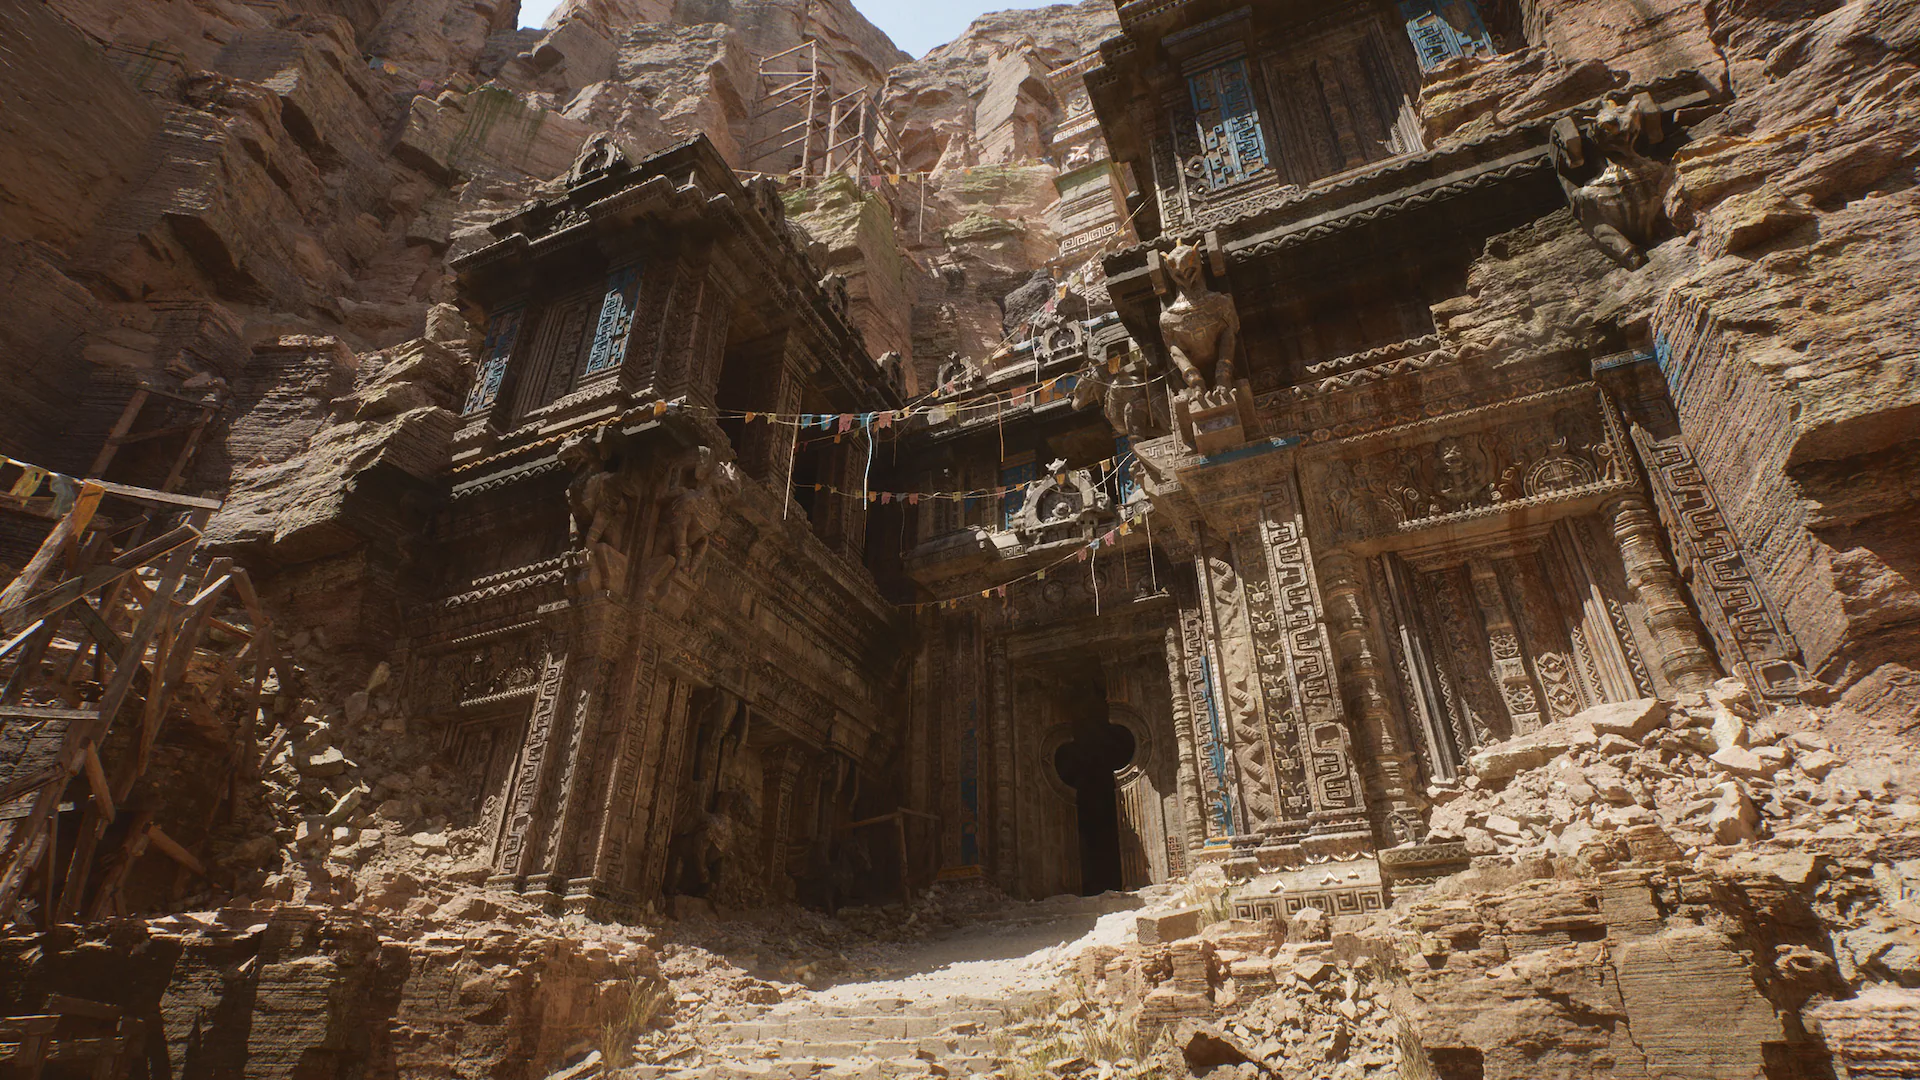
\includegraphics[width=15cm]{images/engines/ue/photorealistic-temple.png}
%     \end{center}
%     \caption{Przykład renderowania hybrydowego w Unreal Engine 5}
%     \label{fig:ue5-photorealistic-temple}
% \end{figure}

% \subsubsection{Filament}
% manual memory management
% good graphics, physically based,
% c++, based
% implies using objective-c in the project
% everything is written in c++
% \begin{figure}[H]
%     \begin{center}
%         \includegraphics[width=7cm]{images/engines/filament/helmet.jpeg}
%     \end{center}
%     \caption{Przykład klatki wygenerowanej przez silnik Filament}
%     \label{fig:filament-helmet}
% \end{figure}

\subsection{Biblioteki natywne}
Alternatywą do multiplatformowych rozwiązań są biblioteki natywne.
Zaliczyć do tej grupy możemy produkty dostępne tylko i wyłącznie na pojedynczej platformie lub te, które dostępne są na wielu, lecz każdy wariant zbudowany jest od początku z myślą o platformie.
Pomimo, że wsparcie pojedynczego środowiska stanowi ograniczenie przez wzgląd na dużo mniejszą grupę odbiorców w stosunku do wieloplatformowych odpowiedników to przynosi także korzyści.
Do najważniejszych zaliczyć możemy możliwość uzyskania optymalnej wydajności, większą intuicyjność wynikającą z możliwości tworzenia interfejsu dostosowanego do przyjętych konwencji.
Dodatkowo, pozwalają na dostęp do wszystkich funkcjonalności platformy i są łatwiejsze w debugowaniu przez wzgląd na fakt, że stworzone są w oparciu o natywne technologie.

\subsubsection{SceneKit}
\begin{figure}
    \begin{center}
        \includegraphics[width=15cm]{images/engines/scene-kit/editor.jpg}
    \end{center}
    \caption{Edytor treści w silniku SceneKit}
    \label{fig:scenekit-editor}
\end{figure}

\begin{figure}
    \begin{center}
        \includegraphics[width=15cm]{images/engines/scene-kit/example-game.jpg}
    \end{center}
    \caption{Przykładowa gra w silniku SceneKit}
    \label{fig:scenekit-example-game}
\end{figure}
Debiut rozwiązania nastąpił w 2012 roku. 
Za projekt i wykonanie odpowiedzialna jest firma Apple, której urządzenia stanowią jedyną docelową grupę odbiorców oprogramowania.
Początkowo wsparcie ograniczało się do platformy OS X, rozszerzenie dostępności na urządzenia mobilne została odroczone do 2014 roku.
Na przestrzeni lat dodano również wsparcie dla watchOS oraz tvOS.
\par
Pragnąc zaklasyfikować SceneKit najtrafniej byłoby określić, iż jest to biblioteka graficzna realizująca dodatkowo pewne funkcjonalności silnika do gier.
Jest to możliwość kontroli audio oraz integracja silnika fizycznego. 
W przeciwieństwie do wiodących rozwiązań skierowanych do branży gier SceneKit nie pozwala na skryptowanie, ani programowanie wizualne.
Niewątpliwą zaletą takiego stanu rzeczy jest znacznie łatwiej użytkownik biblioteki jest w stanie przyswoić sobie możliwości biblioteki.
\par
Myśląc o grupie docelowej wskazać można deweloperów tworzących gry typu indie - w niewielkiej grupie, z małym budżetem.
Ponadto, SceneKit świetnie sprawdza się w roli generatora grafiki trójwymiarowej w aplikacjach innych niż gry wideo.
Z uwagi na fakt, że jest to technologia natywna bardzo łatwo wkomponować można widoki z animowanymi scenami w aplikacje pełniącą inną funkcje niż rozrywkowa.
Sam narzut w kwestii wielkości paczki również jest niewielki, co tylko potwierdza tezę.
% Kod źródłowy projektu nie jest publiczny, jednak uzyskanie dostępu do plików binarnych biblioteki jest darmowe.
% Nie podlega opłacie także wykorzystanie jej we własnym projekcie bez względu czy jego dalsza dystrybucja jest odpłatna.
\par
Nie bez przyczyny wspomniano o dacie wydania biblioteki.
Choć jej interfejs ewoluował i rozrastał się w miarę upływu lat to założenia pozostały niezmienione.
2015 był rokiem kiedy podczas konferencji WWDC Apple zaprezentowało koncepcje, które sugerują programistom wykorzystującym język Swift.
W głównej mierze uogólnić można je na zestaw sugestii, które sprawią, że kod będzie reużywalny, testowalny oraz przejrzysty.
Je same postanowili także wcielić w swoje biblioteki i w miarę uaktualniania języka Swift i tworzenia nowych bibliotek rozszerzających funkcjonalności iOS Apple stawiało na luźne powiązania pomiędzy komponentami i testowalność.
Niestety reforma ta nie dotknęła SceneKit.
\par
2018 rok był ostatnim kiedy wprowadzono usprawnienia do produktu.
Od tamtego czasu użytkownicy nie otrzymali żadnych poprawek, ani stanowiska Apple wyjaśniającego przyszłość projektu.
Sytuację komplikuje fakt, że kod źródłowy jest zamknięty, więc użytkownicy nie są w stanie na własną rękę skorzystać z nowinek technologicznych.
\par
Pomimo, że Apple jest gigantem, ma ogromne dochody i przez wielu programistów traktowane jest jako miejsce w którym jakość jest najważniejsza to nadal w pewnych kwestiach można poczuć się zawiedzionym.
Jednym w takich chwil jest spojrzenie na dokumentację SceneKit.
Przyznać należy, że w sieci dostępnych jest wiele projektów demonstrujących działanie.
Natomiast pozytywny obraz przyćmiewają wszechobecne lakoniczne opisy odnoszące się do zawartości biblioteki.
Niejednokrotnie klasy oraz ich zmienne posiadają wyjaśnienia w formie pojedynczych zdań, nie nadających im szerszego kontekstu.
Odnieść można wrażenie, że jedyną drogą do zrozumienia pewnej puli z zaimplementowanych mechanizmów będzie wysnucie własnych wniosków na podstawie empirycznych doświadczeń.
\subsubsection{ARKit}
Wydanie ARKit było odpowiedzią na rosnące zainteresowanie branży technologią rozszerzonej rzeczywistości.
Idea polega na wzbogacanie obrazu przechwytywanego z kamery urządzenia o dodatkowe elementy 2D oraz 3D.
Podobnie jak w przypadku SceneKit jest to autorska biblioteka Apple.
Choć część funkcjonalności współdzielona jest z SceneKit to firma deklaruje, iż rozwiązania nie są w żadnym stopniu powiązane ze sobą.
\par
ARKit poprawia wiele problemów, które obecne są w SceneKit.
Przede wszystkim jest ona aktywnie rozwijana, na bieżące publikowane są poprawki, a także rozszerzenia funkcjonalności.
Bibliotekę pochwalić należy za ulepszony model oświetlenia i wydajność.
\par
Interfejs ARKit jest kolejnym czynnikiem zaskakującym pozytywnie.
Dostosowany jest on do współczesnych konwencji firmy i dobrze integruje się z resztą systemu.
Tak jak wspomniano wcześniej interakcje oparte o luźne powiązania pozytywnie wpływają na testowalność kodu wykorzystującego bibliotekę.
\par
Podobnie jednak jak w przypadku innych bibliotek Apple ARKit nie jest otwarta.
Nie istnieje możliwość wglądu do kodu, ani jego modyfikacji, jednak technologia może być w nieodpłatny sposób wykorzystana i przeznaczona do celów komercyjnych.
\begin{figure}
    \begin{center}
        \includegraphics[width=15cm]{images/engines/ar-kit/example-app.jpg}
    \end{center}
    \caption{Rzeczywistość rozszerzona na przykładzie aplikacji mobilnej}
    \label{fig:arkit-example-app}
\end{figure}
\par
Zaskakiwać może również, że w ARKit obsługuje jedynie iOS.
Na pozostałych platformach nie występuje lub tak jak przypadku międzyplatformowej technologii \textit{mac catalyst} wywołania są ignorowane.
Z jednej strony to zrozumiałe, ponieważ tylko telefony i tablety posiadają stosowne kamery spełniające wymagania.
Z drugiej wyklucza to możliwość wykorzystania ARKit do użycia w celu wygenerowania prostych scen 3D bez AR.
\subsection{Pozostałe silniki}
W celu dokonania rzetelnej oceny rynku dokonano także przeglądu projektów open source udostępnionych za pomocą platform github.com oraz gitlab.com.
Kryterium, którego spełnienia oczekiwano była dostępność na wszystkie platformy Apple i możliwość uruchomienia biblioteki na najnowszych systemach operacyjnych.
W rezultacie wyszukiwania znaleziono wiele projektów, niestety żaden z nich nie mógł określony być jako stabilne rozwiązanie godne do polecenia.
Natywnych dostępnych było poniżej dziesięciu.
Jako te będące w zaawansowanej formie rozwoju wyróżnić można https://github.com/Hi-Rez/Satin czy https://github.com/Hongtae/SwiftVVD.
\par
Warto wspomnieć, że poza wymienionymi przykładami bibliotek oraz silników istnieje wiele innych alternatyw.
Jako najpopularniejsze można przytoczyć tutaj jmonkey, urho3d, OGRE 3D, Amazon Lumberyard czy panda 3d.
Wszystkie z nich oparte są o podejście open-source.
Były to rozwiązania niegdyś popularne lub stale zwiększające swoje zasięgi jednak ze względu na koncentracja pracy wokół platform Apple wyłączono je z dalszej analizy.
Głównie za sprawą skierowania jedynie na platformy stacjonarne lub wybrakowane wsparcie spowodowane zamknięciem się firmy Apple na API inne niż Metal.
\par
Sytuacja podobnie wygląda w przypadku produkcji takich jak CryEngine, Frostbite, RAGE czy Naughty Dog Game Engine.
Wszystkie z nich cieszą się niemałą popularnością i sukcesem w świecie gier.
Niestety są one skierowane tylko i wyłącznie na stacjonarne platformy.
Dodatkowo, część podlega opłatą licencyjnym, zaś inne nie mogą być w ogóle użyte z uwagi na fakt, że ich źródła są niepubliczne, a pliki binarne dystrybuowane są jedynie do projektów na potrzeby firmy.
